\documentclass[10pt,a4paper]{article}
\usepackage[utf8]{inputenc}
\usepackage{amsmath}
\usepackage{amsfonts}
\usepackage{amssymb}
\usepackage{graphicx}
\usepackage[left=2cm,right=2cm]{geometry}
\usepackage{float}
\usepackage{caption}
\usepackage{subcaption}
\usepackage[hidelinks=true]{hyperref}
\usepackage{lscape}

\title{\bf Model Order Reduction \\ Power Grid Circuit Reduction \\ Final Course Project}
\author{\bf Razvan-Andrei Stoica}
\date{December 3, 2014}

\begin{document}
\maketitle
\begin{abstract}
In this project report we apply the reduction theory studied throughout the course on a power grid circuit. In doing so, we firstly consider a given power grid which we expand by one more layer and then model its state space representation. Having obtained this, we then consider the two reduction methods studied: the balancing transformation and the modal approximation. Our report is thus concluded by a comparison of the two and their accompanying error systems.  
\end{abstract}

\section{Preliminaries}
Model reduction is an essential analysis tool of complex dynamical systems. In the sequel, we considered the following power grid model circuit, Figure (\ref{fig:orig_circ}), as the system to start our analysis with. Our goal was therefore to apply the model reduction methods studied in the course on a similar circuit to the one given, but one layer more complex. Consequently, we firstly expanded the model represented by the circuit in Figure (\ref{fig:orig_circ}) by one more layer, obtaining the circuit in Figure (\ref{fig:circ}), where the original labeling style was preserved. This latter one constituted "the model of analysis" for our project.

\begin{figure}[!ht]
\centering
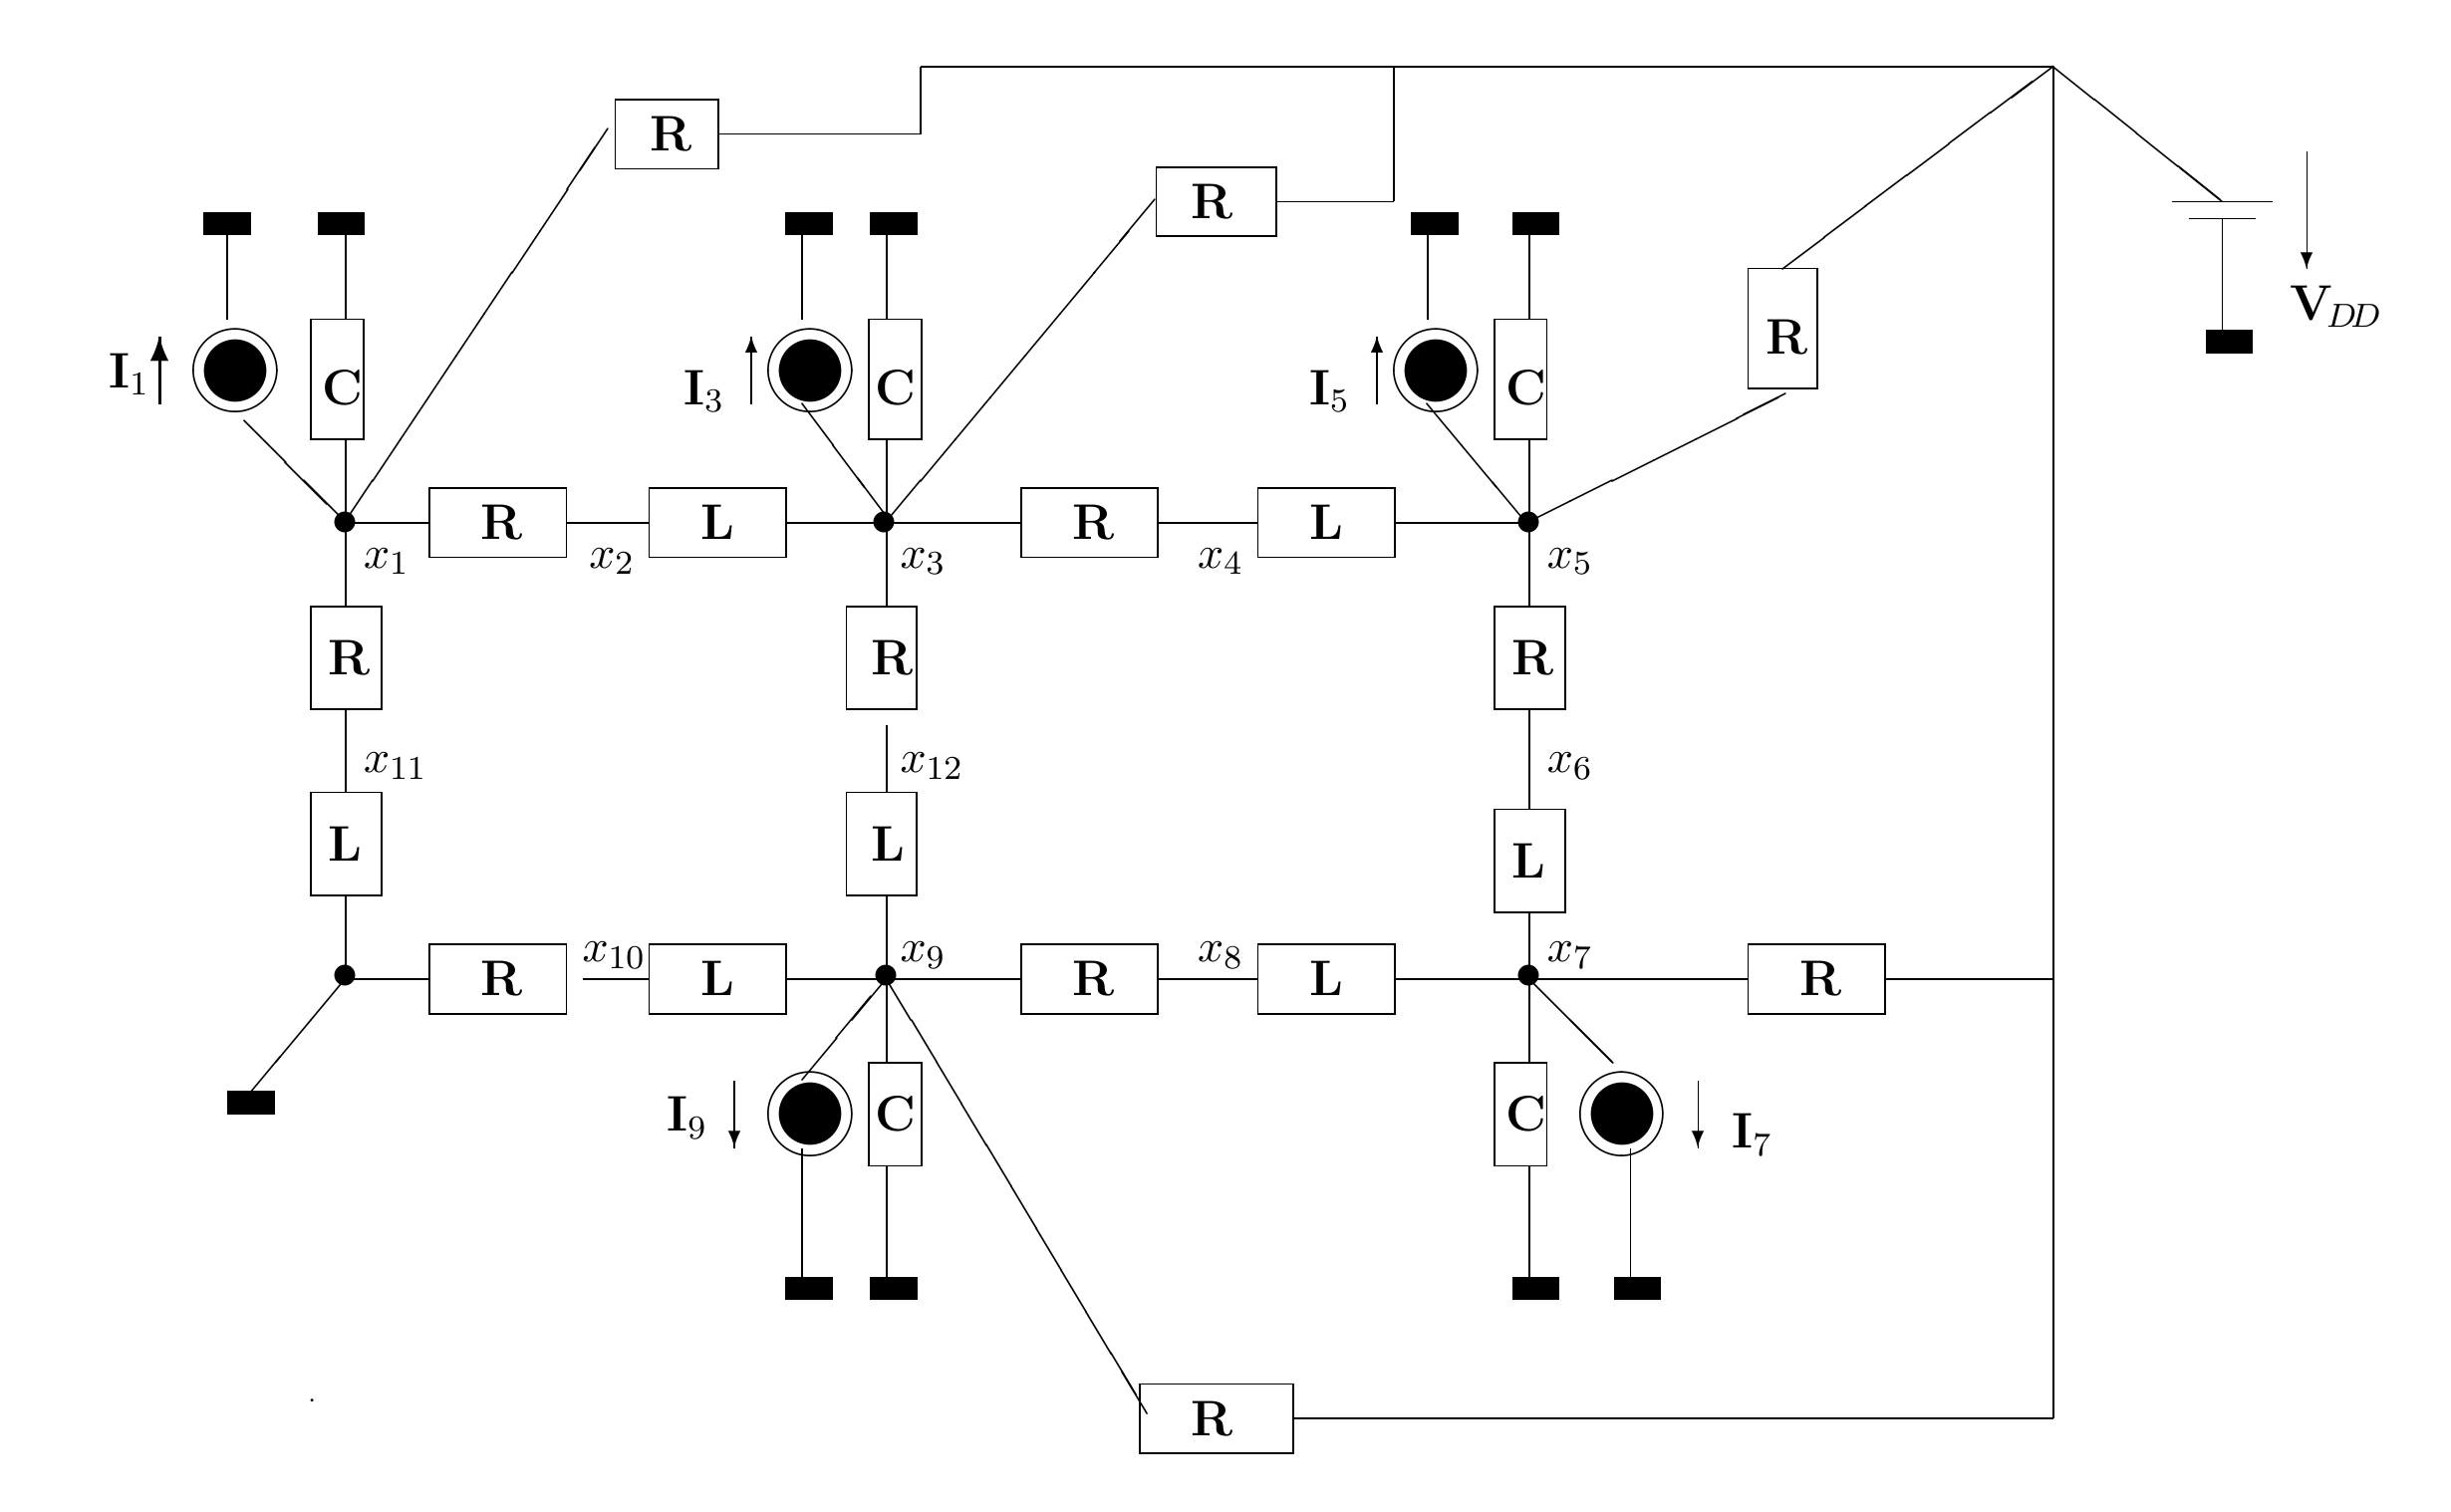
\includegraphics[scale=0.3]{./figs/pwr_grid}
\caption{Initial power grid module circuit with 2 layers ("micro-circuits"), \cite{task}}\label{fig:orig_circ}
\end{figure} 

\begin{figure}[!ht]
\centering
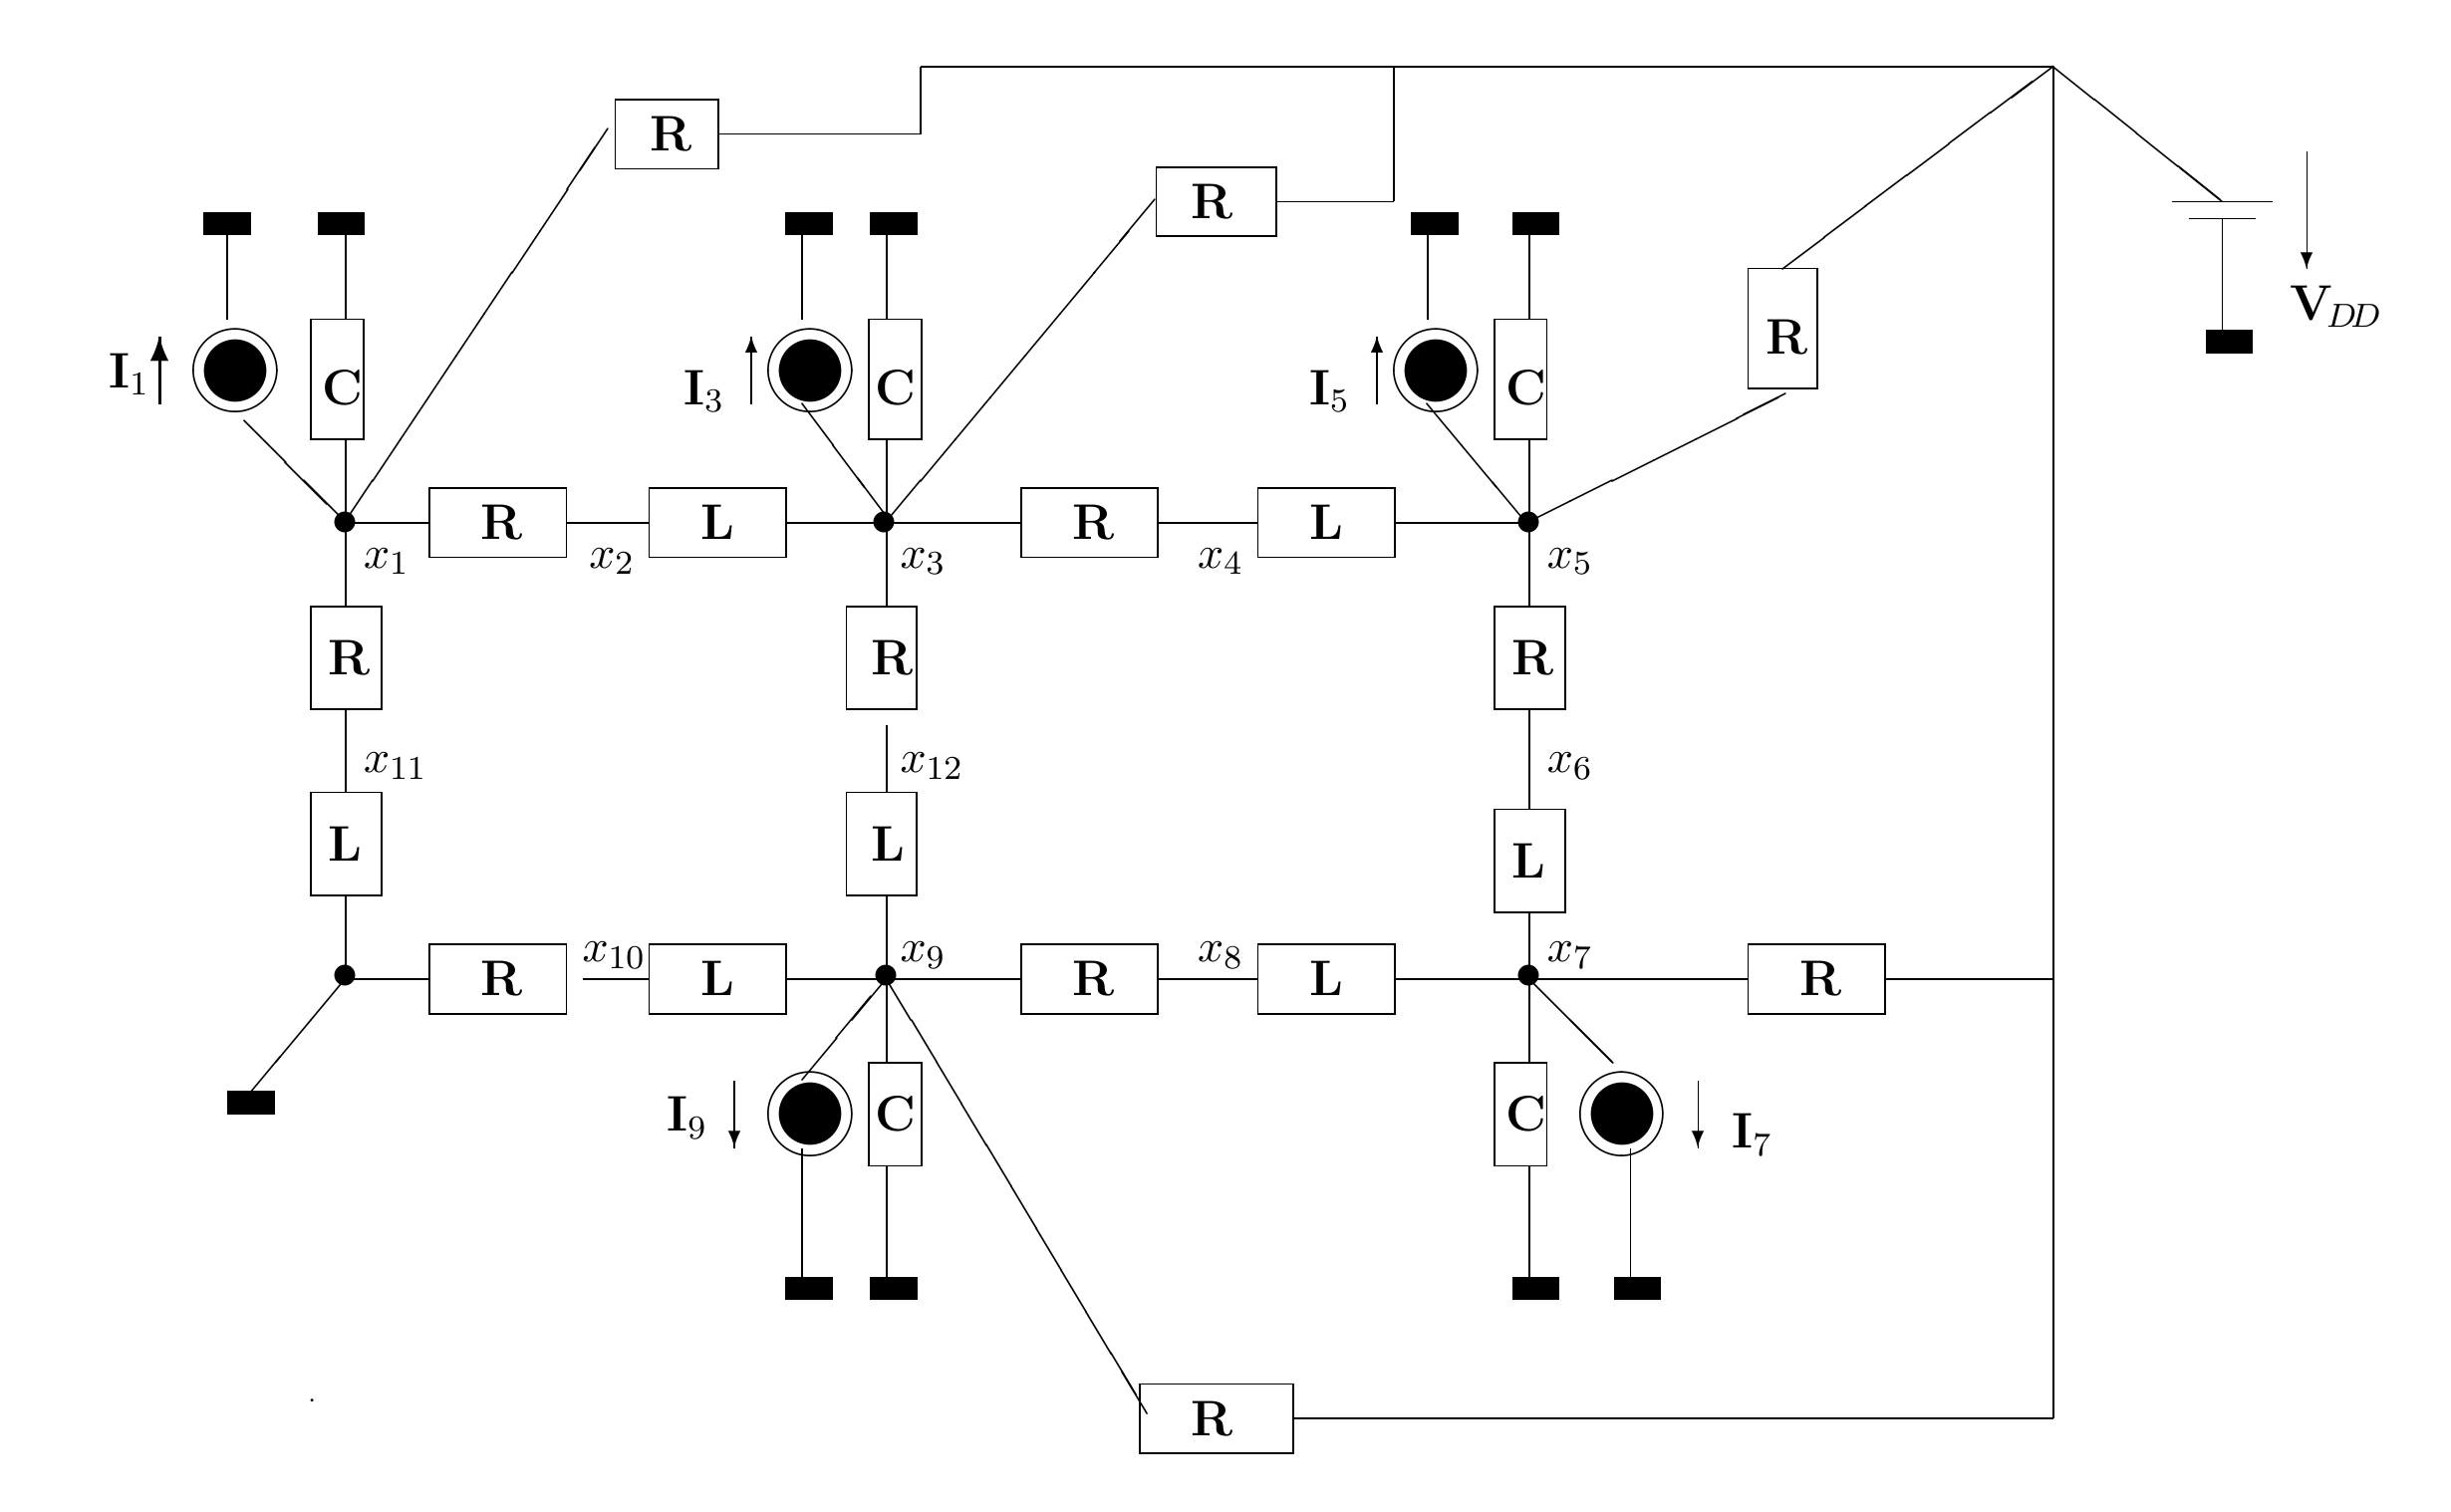
\includegraphics[scale=0.35]{./figs/pwr_grid} % change this to expanded circ.
\caption{Power grid model circuit to study (3 layers)}\label{fig:circ}
\end{figure}

We started by firstly determining the state space representation of the circuit's underlying dynamic system. In doing so, Kirchhoff's laws were applied, and hence, we obtained  the following equations (\ref{eq:sys}).

\begin{eqnarray}\label{eq:sys}
\left\lbrace\begin{array}{c | c}
C\dot{x_1} = -\frac{x_1}{R_1} - x_2 + x_{15} + \frac{u}{R_1} - I_1 & L\dot{x_2} = x_1 - R_2x_2 -x_3\\
C\dot{x_3} = -\frac{x_3}{R_3} + x_2 -x_4 - x_{16} + \frac{u}{R_3} - I_3 & L\dot{x_4} = x_3 - R_4x_4 -x_5\\
C\dot{x_5} = -\frac{x_5}{R_5} + x_4 - x_6 - x_{17} + \frac{u}{R_5} - I_5 & L\dot{x_6} = x_5 - R_6x_6 -x_7\\
C\dot{x_7} = -\frac{x_7}{R_7} +x_6 - x_8 + \frac{u}{R_7} - I_7 & L\dot{x_8} = x_7 - R_8x_8 -x_9\\
C\dot{x_9} = -\frac{x_9}{R_9} + x_8 -x_{10}+ \frac{u}{R_9} - I_9 & L\dot{x_{10}} = x_9 - R_{10}x_{10} -x_{11}\\
C\dot{x_{11}} = \frac{x_{11}}{R_{11}} + x_{10} - x_{12} + x_{17} + \frac{u}{R_{11}} - I_{11} & L\dot{x_{12}} = x_{11} - R_{12}x_{12} -x_{13}\\
C\dot{x_{13}} = -\frac{x_{13}}{R_{13}} + x_{12} - x_{14} + x_{16} + \frac{u}{R_{13}} - I_{13} & L\dot{x_{14}} = x_{13} - R_{14}x_{14}\\
& L\dot{x_{15}} = -x_1 - R_{15}x_{15} \\
&L\dot{x_{16}} = x_3 - R_{16}x_{16} -x_{13}\\
&L\dot{x_{17}} = x_5 - R_{17}x_{17} -x_{11}\\
\end{array}\right.
\end{eqnarray}

Rewriting equations (\ref{eq:sys}) in state-space form

\begin{eqnarray}
\begin{array}{c c}
\dot{\textbf{x}} = & A \textbf{x} + B \textbf{u}\\
\textbf{y} = & C\textbf{x} +  D\textbf{u},\nonumber
\end{array}
\end{eqnarray}

we obtained the following input, state and output column vectors

\begin{equation}
\textbf{u} = \left(I_1, I_2, I_3, \dots, I_7, V_{DD}\right)^T\nonumber
\end{equation}

\begin{equation}
\textbf{x} = \left(x_1, x_2, x_3, \dots, x_{16}, x_{17}\right)^T\nonumber
\end{equation}

\begin{equation}
\textbf{y} = \left(y_1, y_2, y_3, \dots, y_{7}\right)^T\nonumber
\end{equation}
using the same notation introduced in Figure (\ref{fig:circ}) for the input, and respectively, for the state vectors, while the output was just defined as a $7$-length vector in order to outline the dimensionality of the system. Hence, it was clear that our dynamic system had $m = 8$ inputs, $n = 17$ states and $p = 7$ outputs. Furthermore, the matrices $A, B, C$ and $D $ which defined the system are shown in (\ref{eq:A})-(\ref{eq:D}). 

\begin{landscape}
\begin{equation}\label{eq:A}
A =\left(\begin{array}{c c c c c c c c c c c c c c c c c c}
-\frac{1}{R_1} & -1 & 0 & 0 & 0 & 0 & 0 & 0 & 0 & 0 & 0 & 0 & 0 & 0 & 1 & 0 & 0\\
1 & -R_2 & -1 & 0 & 0& 0 & 0 & 0& 0 & 0 & 0 & 0 & 0 & 0 & 0 & 0 & 0\\
0 & 1 & -\frac{1}{R_3} & -1 & 0 & 0 & 0 & 0 & 0 & 0 & 0 & 0 & 0 & 0 & 0 &-1 & 0  \\
0 & 0 & 1 & -R_4 & -1 & 0 & 0 & 0 & 0 & 0 & 0 & 0 &0 & 0& 0& 0& 0\\
0& 0 & 0 & 1 & -\frac{1}{R_5} & -1 & 0 & 0 & 0 & 0 & 0 & 0 & 0 &0 & 0& 0& -1\\
0& 0 & 0 & 0 & 1& -R_6 & -1 & 0 & 0 & 0 & 0 & 0 & 0 & 0 &0 & 0& 0\\
0& 0 & 0 & 0 & 0 & 1& -\frac{1}{R_7} & -1 & 0 & 0 & 0 & 0 & 0 & 0 & 0 &0 & 0\\
0& 0 & 0 & 0 & 0 & 0& 1& -{R_8} & -1  & 0 & 0 & 0 & 0 & 0 & 0 &0 & 0\\
0& 0 & 0 & 0 & 0 & 0& 0& 1& -\frac{1}{R_9} & -1  & 0 & 0 & 0 & 0 & 0 &0 & 0\\
0& 0 & 0 & 0 & 0 & 0& 0& 0& 1& -{R_{10}} & -1  & 0 & 0 & 0 & 0 &0 & 0\\
0& 0 & 0 & 0 & 0 & 0& 0& 0& 0 & 1& -\frac{1}{R_{11}} & -1  & 0 & 0 & 0 & 0 &1 \\
0& 0 & 0 & 0 & 0 & 0& 0& 0& 0 & 0& 1& -{R_{12}} & -1  & 0 & 0 & 0 & 0 \\
0& 0 & 0 & 0 & 0 & 0& 0& 0& 0 & 0& 0& 1& -\frac{1}{R_{13}} & -1  & 0 & 1 & 0 \\
0& 0 & 0 & 0 & 0 & 0& 0& 0& 0 & 0& 0& 0& 1& -{R_{14}} & 0 & 0 & 0 \\
-1& 0 & 0 & 0 & 0 & 0& 0& 0& 0 & 0& 0& 0& 0& 0& -{R_{15}} & 0 & 0 \\
0& 0 & 1 & 0 & 0 & 0& 0& 0& 0 & 0& 0& 0& -1& 0& 0& -{R_{16}} & 0 \\
0& 0 & 0 & 0 & 1 & 0& 0& 0& 0 & 0& -1& 0& 0& 0& 0& 0& -{R_{17}} \\
\end{array}\right)
\end{equation}

\begin{equation}\label{eq:B}
B = \left(\begin{array}{c c c c c c c c c c c c c c c c c}
-1 & 0& 0 & 0 & 0 & 0& 0& 0& 0& 0 & 0 & 0 & 0& 0& 0& 0& 0 \\
0 & 0& -1 & 0 & 0 & 0& 0& 0& 0& 0 & 0 & 0 & 0& 0& 0& 0& 0 \\
0 & 0& 0 & 0 & -1 & 0& 0& 0& 0& 0 & 0 & 0 & 0& 0& 0& 0& 0 \\
0 & 0& 0 & 0 & 0 & 0& -1& 0& 0& 0 & 0 & 0 & 0& 0& 0& 0& 0 \\
0 & 0& 0 & 0 & 0 & 0& 0& 0& -1& 0 & 0 & 0 & 0& 0& 0& 0& 0 \\
0 & 0& 0 & 0 & 0 & 0& 0& 0& 0& 0 & -1 & 0 & 0& 0& 0& 0& 0 \\
0 & 0& 0 & 0 & 0 & 0& 0& 0& 0& 0 & 0 & 0 & -1& 0& 0& 0& 0 \\
-\frac{1}{R_1} & 0& -\frac{1}{R_3} & 0 & -\frac{1}{R_5} & 0& -\frac{1}{R_7}& 0& -\frac{1}{R_{11}}& 0 & -\frac{1}{R_{13}} & 0 & 0& 0& 0& 0& 0 \\
\end{array}\right)^T
\end{equation}

\begin{equation}\label{eq:C}
C = B(:,1:7)',
\end{equation}
using MATLAB notation.

\begin{equation}\label{eq:D}
D = \text{zeros}(7,8),
\end{equation}
using MATLAB notation
\end{landscape}

It is easy to see that the sparse system matrix $A$ maintains the structure of the one representing the two-layered system we initially started with. This is an expected result common for such grid circuits.

Finally, before starting our analysis for reduction, we considered the values
$C_i = L_j = 1$ in their expected unit of measure, and respectively, $R_1 = R_{13} = 0.01 \Omega$, $R_2 =  R_4 = R_6 = R_8 = R_{10} = R_{12} = R_{14} = 2\Omega$ and $R_3  = R_5 = R_7 = R_9 = R_{11} = 100 \Omega$, $R_{15} = R_{16} = 3 \Omega$, and $R_{17} = 4 \Omega$, extrapolating the example given in \cite{task}. As a consequence, we found and defined our system to work with.

\section{Model reduction methods}
Having found the state space representation of our system, we proceeded with the model reduction using two methods: \textit{balanced truncation} and \textit{modal approximation}. In the following subsection a short theoretical background on the two methods is given together with the algorithms we used to obtain the reduction on our system using MATLAB.

\subsection{Balanced truncation}
Any linear dynamic system $\Sigma := (A,B,C,D)$ can be transformed to a balanced representation $\Sigma_{bal} := (T_{bal}AT^{-1}_{bal},T_{bal}B,CT_{bal}^{-1},D)$, where the infinite controllability, and respectively, observability Grammians are of the original system transform by congruence to diagonal and equal, i.e. "balanced", matrices, $T_{bal}PT_{bal}* =: P_{bal} = Q_{bal} := T_{bal}^{-*}QT_{bal}^{-1}$. 

Moreover, the diagonal entries of $P_{bal}, Q_{bal}$, $\sigma_1 \geq \sigma_2 \geq  ... \geq \sigma_n\geq 0$ are the Hankel singular values of the system (eigenvalues of the product matrix $PQ$) and they order simultaneously the reachable and observable states of the system quantitatively such that the most reachable state is at the same time also the most observable. Consequently, this yields a high quality reduction capability and this is achieved by simply discarding the Hankel singular values that  fall under a certain threshold. Furthermore, balanced truncation up to an order $k \leq n$ returns a reduced system which is controllable ($\sigma_k > 0$), observable ($\sigma_k > 0$) and stable (stability of original system preserved through similarity transform of matrix $A$).

The procedure to determine the balancing transformation matrix $T_{bal}$ is as follows:
\begin{itemize}
\item [1.] if system $\Sigma$ is stable
\item [2.] \hspace{0.3cm} compute infinite Gramian controllability matrix $P$ as solution to Lyapunov's equation $$AP^T+PA^T+BB^T = 0$$
\item [3.] \hspace{0.3cm} compute infinite Gramian observability matrix $Q$ as solution to Lyapunov's equation $$A^TQ+Q^TA+C^TC = 0$$
\item [4.]\hspace{0.3cm} solve EVD of $$Q^{\frac{1}{2}}PQ^{\frac{1}{2}} = VH_DV^*,$$ and get the squared Hankel singular values as descendingly ordered diagonal entries in $H_D$ and $V$ the transformation matrix.
\item[5.] \hspace{0.3cm} determine the balancing transformation matrix $$T_{bal} = H_D^{-\frac{1}{4}}V^*Q^{\frac{1}{2}}$$ and transform $(A,B,C,D) \rightarrow (A_{bal}, B_{bal}, C_{bal}, D_{bal})$.
\item[6.] \hspace{0.3cm} pick truncation order $k$ such that $\sigma_k \geq t$, where $t$ is a considered threshold for truncation, and then, truncate such that $A^k_{bal} := A_{bal}(1:k,1:k)$, $B^k_{bal} := B_{bal}(1:k,:)$, $C^k_{bal} := C_{bal}(:,1:k)$, $D^k_{bal}:=D_{bal}$ in MATLAB notation.   
\end{itemize}

\subsection{Modal approximation}
Any linear dynamic system $\Sigma := (A,B,C,D)$ with a diagonalizable matrix $A$ can be transformed to a modal representation $\Sigma_{mod}:=(\Lambda_A,B_{mod},C_{mod},D_{mod})$, where $\Lambda_A$ is the diagonalized transformation of $A$, i.e $A = V\Lambda_AV^{-1}$ with, and respectively $B_{mod} := V^{-1}B$, $C_{mod} := CV$, $D_{mod} := D$. We consider the diagonalization to sort the eigenvalues ascendingly after their real part, such that for a stable system, i.e. $\text{Re}(\lambda_i )_{i=1,...,n}<0$, $0 \leq \text{Re}(\lambda_1)  \leq \text{Re}(\lambda_2) \leq ... \leq \text{Re}(\lambda_n)$. In this case, since the frequency modes of the systems are preserved and sorted, we could exclude the ones having a small influence, obtaining an approximation which maintains stability of the original system.

The reduction is performed based not only on the real parts of the eigenvalues, but also the influence of the residuals coming from the frequency response is taken into consideration for a lower approximation error, hence we sort the values $\frac{\textbf{c}_{mod,i}\textbf{b}_{mod,i}^T}{\text{Re}(\lambda_i)}_{i=1,...,n}$, with $\textbf{c}_{mod,i}, \textbf{b}_{mod,i}$ taken as column vectors in $C_{mod}$,  and respectively in $B_{mod}$ and then pick the $k^{th}$ of them which are highest than a certain threshold. Consequently we approximate the system with a $k$-order one with same dominant modal properties.

The procedure to achieve modal truncation that we implemented in MATLAB is summarized below:
\begin{itemize}
\item [1.] solve the eigenvalue, eigenvector problem for $A$, i.e. $$ A = V\Lambda_AV^{-1}$$
\item [2.] compute the modal transformed equivalent system $\Sigma_mod$ using $V$
\item [3.] compute the modal weighted coefficients $$m_i := \frac{\textbf{c}_{mod,1}\textbf{b}_{mod,1}^T}{\text{Re}(\lambda_i)}_{i=1,...,n}$$ and sort them ascendingly.
\item [4.] pick the $k$ best coefficients and their corresponding eigenvalues and extract the corresponding matrices $A_{mod}^k$, $B_{mod}^k$, $C_{mod}^k$ by either recomputing with shuffled $V$ or by mere extraction of columns / rows.
\end{itemize}

\section{Model analysis \& reduction}
In our analysis of the model introduced in Section 1, we used both methods summarized in Section 2 for different thresholds levels such as: $10^{-2}, 0.5\cdot10^{-2}, 10^{-3}$. The most interesting results and their comparisons are presented below, while the conclusions are drawn in the end.

\subsection{General analysis}
Prior to the reduction step, we determined whether or not we have to deal with a stable system or not. We did so by analyzing the eigenvalues of the matrix $A$, which were in fact the poles, or the modes, of our system. Thus, we solved the eigendecomposition of $A$ and obtained that all the poles were in the left half plane (see Figure ()). Consequently, the system was stable, and since $A$ was also diagonalizable,  we could directly apply both methods of approximation we have previously described without any problems. 

In addition, we computed the controllability matrix $R_{n=17}(A,B)$ and the observability matrix $O_{n=17}(C,A)$, and then we determined their singular values in order to determine their ranks. The computation yielded that the singular values of the controllability matrix $R$ were $\sigma^{R}_i \geq 7.6576\cdot10^3 > 0$, and respectively that the  singular values of the observability matrix $O$ were $\sigma^{O}_i \geq 2.2413\cdot10^3 > 0$, and as a consequence both matrices were full rank and hence the system was both controllable and observable. Consequently, we had to analyze a \textbf{stable, controllable} and \textbf{observable} dynamic linear system.

\subsection{System order reduction}
In preparation for the reduction step using the two methods outlined, we computed the normalized Hankel singular values $\frac{\sigma_k}{\sigma_1}$, and respectively, the normalized modal coefficients $\frac{m_{k}}{m_{1}}$, for $k\leq n$, and then we plotted the results, see Figure (\ref{fig:svc_vs_k}).

\begin{figure}[!ht]
\centering
\includegraphics[scale=0.5]{./figs/hsv_modc_vs_k}
\caption{Normalized Hankel singular values and normalized modal coefficients vs. system order $k$}\label{fig:svc_vs_k}
\end{figure}

Figure (\ref{fig:svc_vs_k}) already provides quite some insight into the approximation capabilities of the reduced systems. For example, we remark the sudden drop after the first coefficient and then the flat regions for both methods up to $k = 9$ order. Around this region, the threshold value range suggested as a good candidate for our reduction problem, \cite{task}, is also situated. As a result, we ran three different reduction experiments, obtaining different reduced orders for them, see Table (\ref{tab:red}).

\begin{table}[!ht]
\centering
\begin{tabular}{|c | c | c |}\hline
Threshold $tol$ & Reduction order balanced transf. & Reduction order modal approx.\\\hline
$10^{-2}$ & $7$ & $9$\\\hline
$5\cdot10^{-3}$ & $ 8$ & $10$ \\\hline
$10^{-3}$ & $11$& $12$\\\hline 
\end{tabular}
\caption{Reduction order for the balanced truncation and modal approximation given a threshold value}\label{tab:red}
\end{table}

However, given our problem and the plot from Figure (\ref{fig:svc_vs_k}), we will present in this report the required plots only for the last threshold considered as it was the most representative and also the most accurate by some distance with respect to the other two experimented. Nonetheless, the error norms of all the systems were computed and are tabulated at the end of this section.

As a consequence, we reduced the initial system to a balanced transformed reduced system $\Sigma^{(11)}_{bal}$, and respectively to a modal approximated system $\Sigma^{(12)}_{mod}$. Furthermore, in order to observe how the transformation and truncation affected the modes of the original system, we plotted poles of the original system against the poles of the reduced systems. The plot is rendered in Figure (\ref{fig:poles}), where Subfigure (\ref{fig:poles_full}) shows all the poles of the systems, and respectively, where Subfigure (\ref{fig:poles_zoom}) shows a zoomed in version focusing on the poles that are more significant ($\text{Re}(\lambda_i)$ closer to $0$).

\begin{figure}
\centering
\begin{subfigure}{.5\textwidth}
  \centering
  \includegraphics[width=.95\linewidth]{./figs/poles_full}
  \caption{Full spread of poles --- including the two high poles at $-99.9795$ and $-99.9692$ of the original system plus the one at $-99.9741$ of the balancing reduced system}\label{fig:poles_full}
\end{subfigure}%
~
\begin{subfigure}{.5\textwidth}
  \centering
  \includegraphics[width=.95\linewidth]{./figs/poles_zoom}
  \caption{Zoomed in poles comparison --- most significant poles only with two poles close by identifiable almost as one for the original system at $-2.0015$ and at $-2.0124$}\label{fig:poles_zoom}
\end{subfigure}
\caption{Comparison of poles of original system versus reduced approximant systems}\label{fig:poles}
\end{figure}

From the plots of the poles, we remark that indeed the modal approximation keeps the poles of the system unchanged (as the yellow dots hit the center of the blue ones as expected) since this transformation diagonalizes $A$ preserving its eigenvalues even after reduction. On the other hand, the balancing transformation preserves the eigenvalues of the original $A$ through a similarity transformation, but after reduction these eigenvalues are not preserved anymore, drifting apart from their position as the matrix $A$ is not diagonalized by the balancing transformation and hence eigenvectors are not decoupled anymore, which yields these small differences in between the expected pole values and ones after the reduction of the balanced transformation. Hence, both methods preserve the original system's stability property.

Furthermore, we remark that indeed the modal approximant tends to maintain the poles of the systems close to the real axis on the negative side as those are the significant ones for the transfer function of the system. Rarely happens that the residuals play a role for the poles of the reduced system, but even so, we observe this behavior in Subfigure (\ref{fig:poles_zoom}) for the poles further apart from the real axis, where this kind of behavior mind be expected. The balancing transformation keeps the poles that ensure that the easiest states to reach are also the easiest to observe. Of course most of them are the ones closer to the real axis, see Subfigure (\ref{fig:poles_zoom}), but there might also be poles further apart from the real axis, as in for the pole at $-99.9741$, see Subfigure (\ref{fig:poles_full}).



\begin{thebibliography}{3}
\bibitem {aa} A. Antoulas, Lecture Notes Model Order Reduction Course, Fall 2014, Jacobs University Bremen.
\bibitem {task} A. Antoulas, Project guide , Model Order Reduction Course, Fall 2014, Jacobs University Bremen.
\bibitem {matlab} MATLAB online documentation for Control System Toolbox and Robust Control Toolbox, \url{http://de.mathworks.com/help/index.html}.
\bibitem {code} MATLAB project code, Github repository: \url{https://github.com/rstoica/mor_proj} as of December 3, 2014.
\end{thebibliography}
\end{document}